\begin{figure*}
  \centering
  \begin{subfigure}[b]{0.05\textwidth}
    ~
  \end{subfigure}
  % 
  \begin{subfigure}[b]{0.45\textwidth}
    \centering
    ~~\textbf{Mild plate effects}
  \end{subfigure}
  % 
  \begin{subfigure}[c]{0.45\textwidth}
    \centering
    ~~\textbf{Strong plate effects}
  \end{subfigure}

  \begin{subfigure}[c]{0.05\textwidth} 
    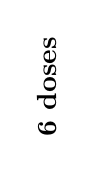
\begin{tikzpicture}
      \node[rotate=90] {\textbf{6 doses}};  
    \end{tikzpicture}
  \end{subfigure}  
  %
  \begin{subfigure}[c]{0.45\textwidth}
    \includegraphics[width=\textwidth]{figures/dose-response-d_diff-1-2-3-6doses-dil18-bowl-neg-controls-0.055.png}
    %\caption{d diff 6doses-dil8-bowl-0.055}
    % \label{fig:tem}
  \end{subfigure}
  %
  \begin{subfigure}[c]{0.45\textwidth}
    \centering
    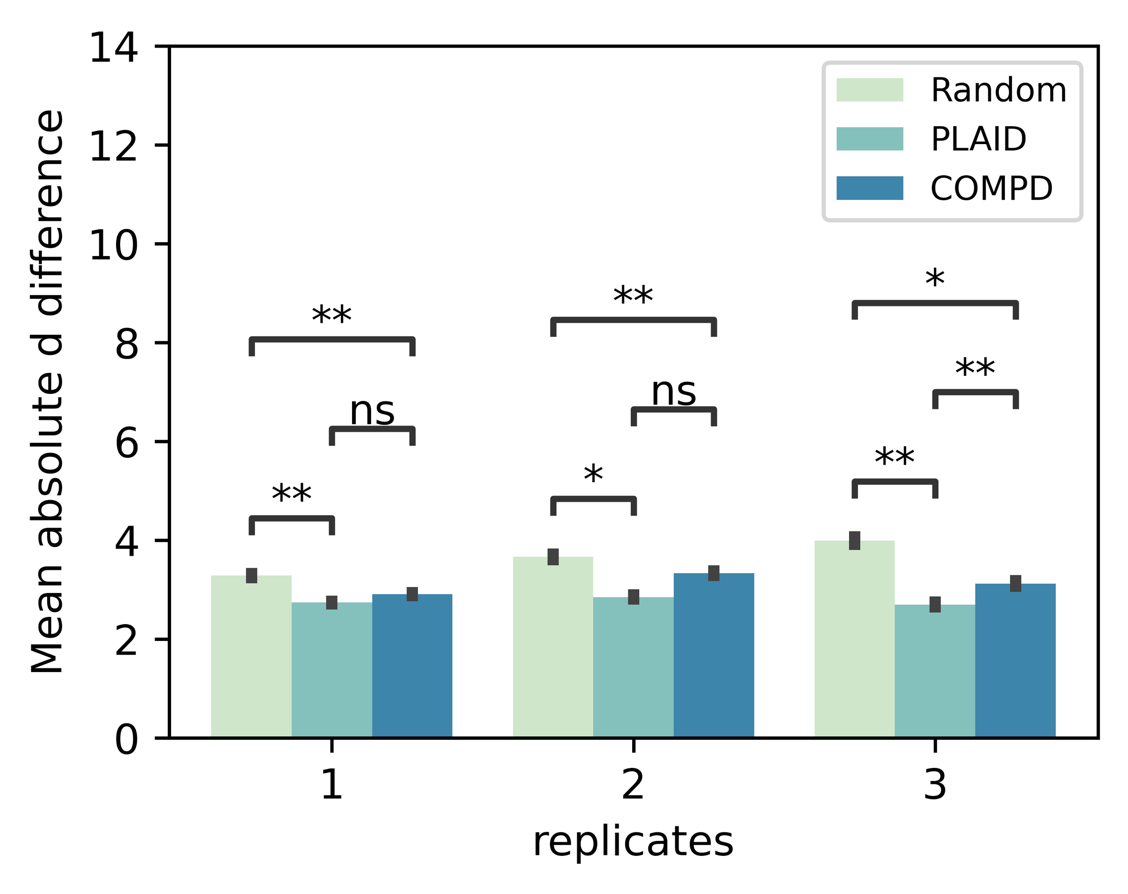
\includegraphics[width=\textwidth]{figures/dose-response-d_diff-1-2-3-6doses-dil18-bowl-neg-controls-0.085.png}
    %\caption{d diff 6doses-dil18-bowl-0.085}
    % \label{fig:tem}
  \end{subfigure}

  \begin{subfigure}[c]{0.05\textwidth}
    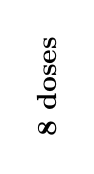
\begin{tikzpicture}
      \node[rotate=90] {\textbf{8 doses}};  
    \end{tikzpicture}
  \end{subfigure}  
  %
  \begin{subfigure}[c]{0.45\textwidth}
    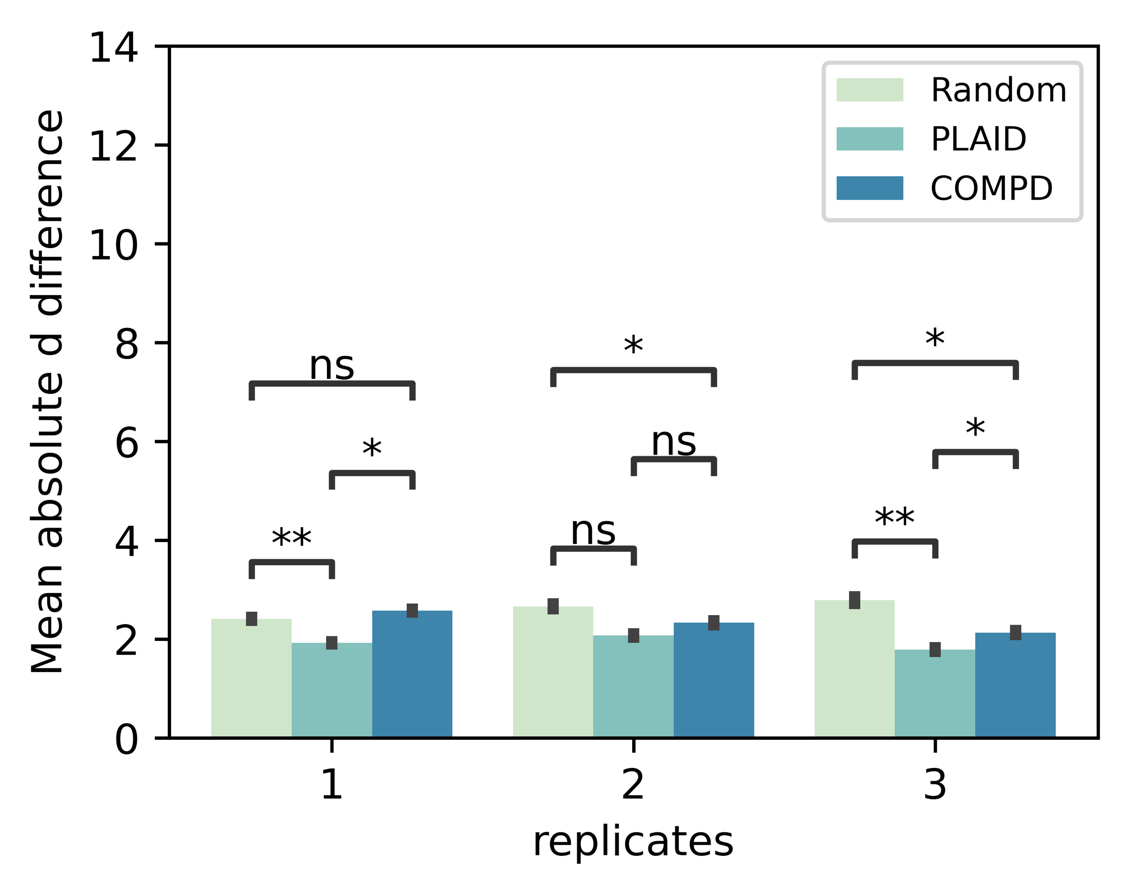
\includegraphics[width=\textwidth]{figures/dose-response-d_diff-1-2-3-8doses-dil8-bowl-neg-controls-0.055.png}
    %\caption{d diff 8doses-dil8-bowl-0.055}
    % \label{fig:tem}
  \end{subfigure} 
  %
  \begin{subfigure}[c]{0.45\textwidth}
    \centering
    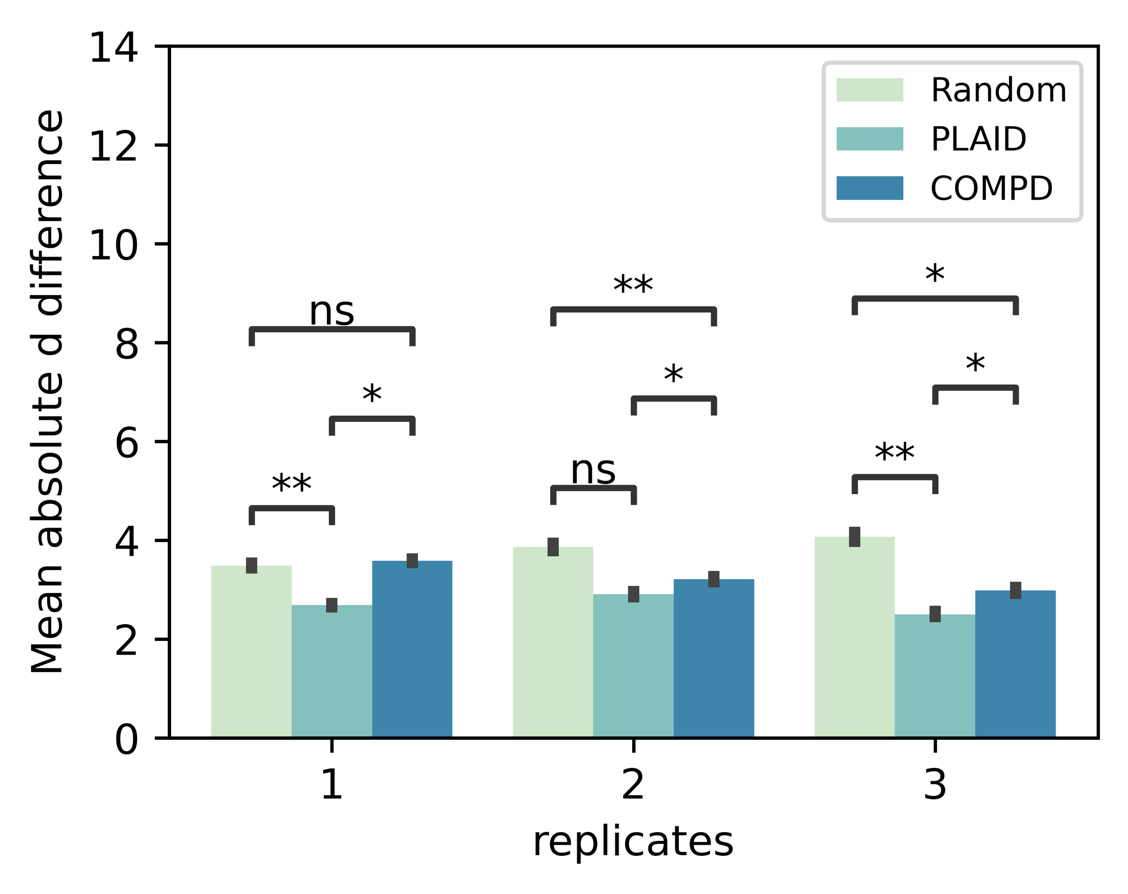
\includegraphics[width=\textwidth]{figures/dose-response-d_diff-1-2-3-8doses-dil8-bowl-neg-controls-0.085.png}
    %\caption{d diff 8doses-dil8-bowl-0.085}
    % \label{fig:tem}
  \end{subfigure}

  \begin{subfigure}[c]{0.05\textwidth}
    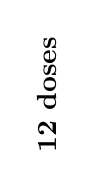
\begin{tikzpicture}
      \node[rotate=90] {\textbf{12 doses}};
    \end{tikzpicture}
  \end{subfigure}  
  % 
  \begin{subfigure}[c]{0.45\textwidth}
    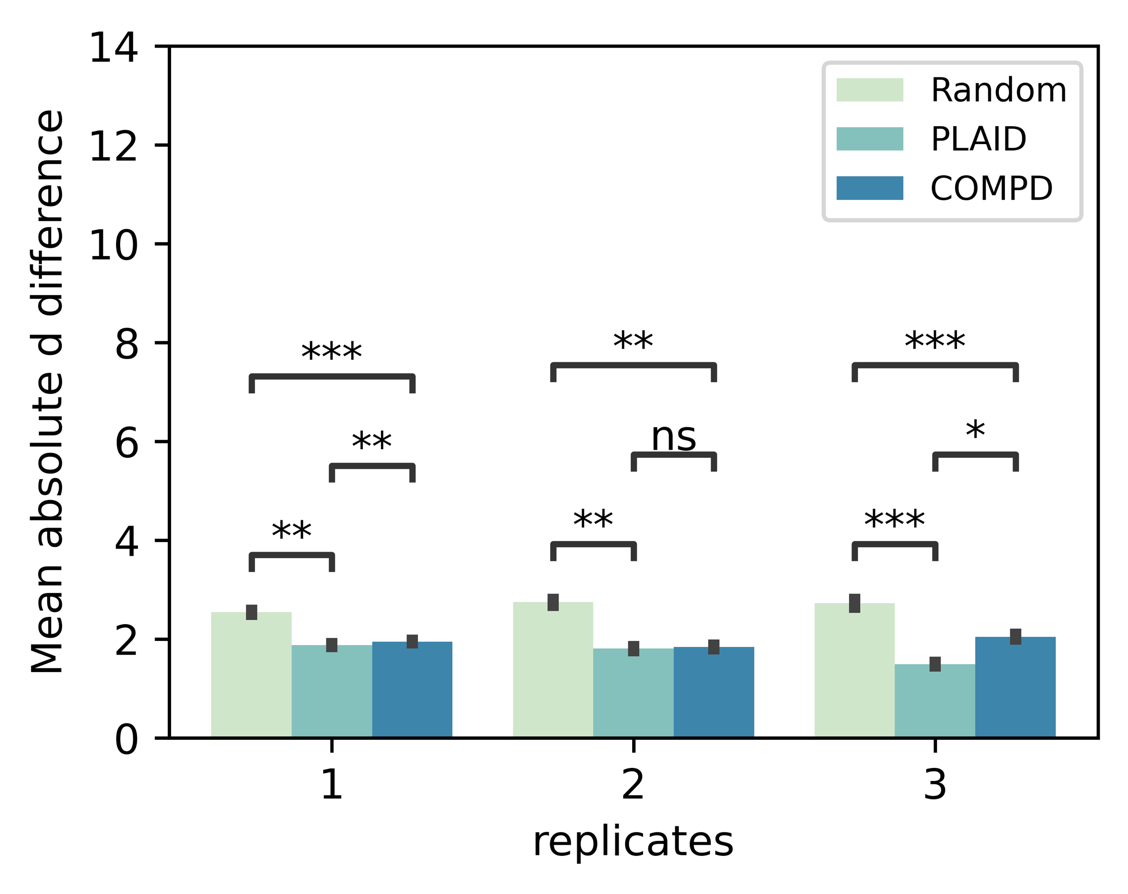
\includegraphics[width=\textwidth]{figures/dose-response-d_diff-1-2-3-12doses-dil4-bowl-neg-controls-0.055.png}
    %\caption{d diff 12doses-dil4-bowl-0.055}
    % \label{fig:tem}
  \end{subfigure} 
  %
  \begin{subfigure}[c]{0.45\textwidth}
    \centering
    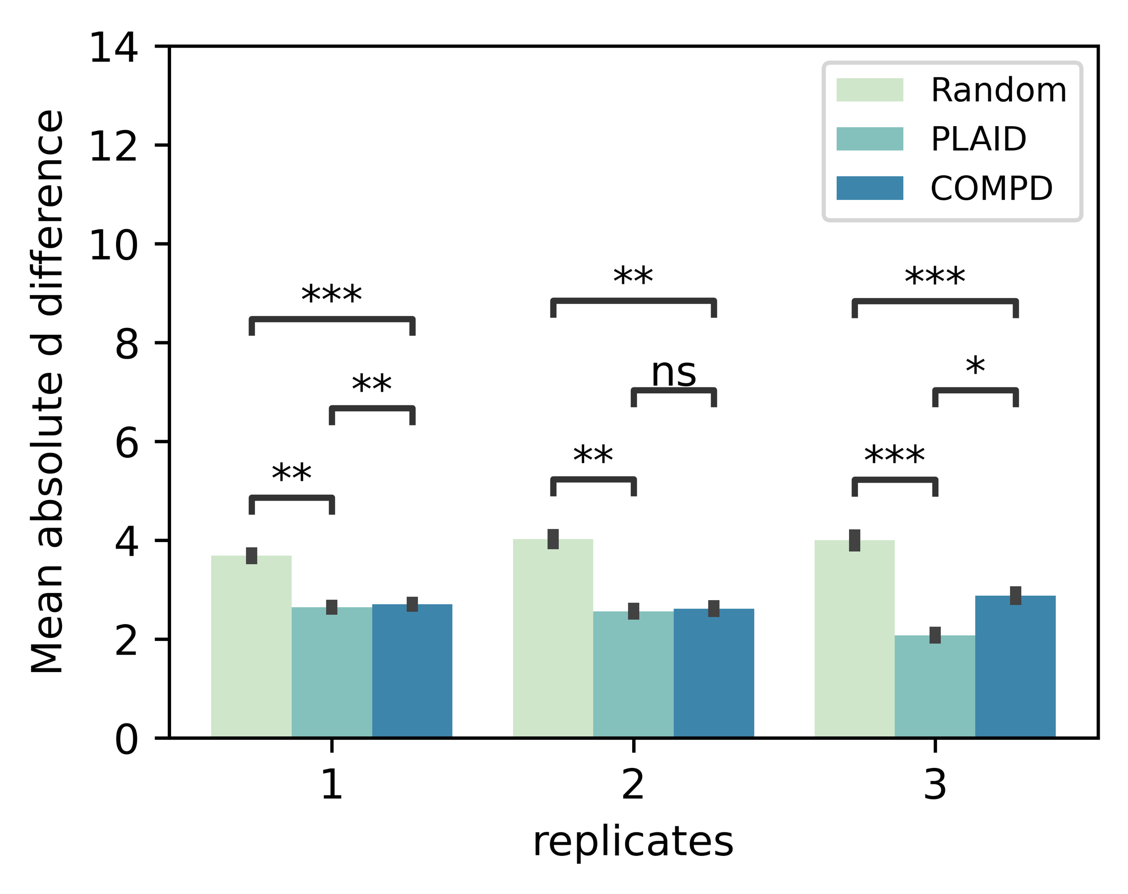
\includegraphics[width=\textwidth]{figures/dose-response-d_diff-1-2-3-12doses-dil4-bowl-neg-controls-0.085.png}
    %\caption{d diff 12doses-dil4-bowl-0.085}
    % \label{fig:tem}
  \end{subfigure}
  \caption{Mean absolute difference between expected and obtained
    heights (max value) for dose-response curves using various numbers
    of doses, replicates, and bowl-shaped plate-effect strengths. The
    4PL sigmoide curves were fitted using compound data and 4 negative
    controls such that their mean was equal to the mean of the 20
    negative controls the plate. *** indicates $p\leq10^{-43}$.}
\end{figure*}


%%% Local Variables: 
%%% mode: latex
%%% TeX-master: "supplement.tex"
%%% End: 